\documentclass[11pt]{article}
\usepackage[margin=1in]{geometry}
\usepackage{amsmath,amssymb,amsthm}
\usepackage{booktabs}
\usepackage{graphicx}
\usepackage{tikz}
\usetikzlibrary{quantikz2,calc}
\colorlet{cnew}{blue!60!cyan!80!black}
\tikzset{muxctrl/.style={minimum width=6pt, minimum height=6pt, inner sep=0pt},
  newgate/.style={fill=cnew!12, draw=cnew, thick},
  wirethru/.style={draw=none, fill=none, append after command={\pgfextra{\draw[line width=0.6pt]
    ([xshift=-0.5pt]\tikzlastnode.west) -- ([xshift=0.5pt]\tikzlastnode.east);}}}}
\usepackage{float}
\usepackage[colorlinks=true,linkcolor=blue!50!black,citecolor=blue!50!black,urlcolor=blue!50!black]{hyperref}

\renewcommand{\thesection}{\Roman{section}}
\renewcommand{\thesubsection}{\thesection.\Alph{subsection}}

\title{Fewer CX gates for exact unitary synthesis via single-qubit pivots}
\author{Matt Bowring\\[2pt]
{\normalsize Purdue University}\\[2pt]
{\normalsize\href{mailto:mbowring@purdue.edu}{\texttt{mbowring@purdue.edu}}}}
\date{October 14, 2026}

\begin{document}
\maketitle

\begin{abstract}
This paper presents an improved quantum gate decomposition that results in smaller quantum circuits.
The current best-known exact decomposition requires $O(\frac{22}{48} 4^n)$ two-qubit gates for an arbitrary $n$-qubit unitary. I reduce this count to $O(\frac{21}{48} 4^n)$ by introducing a parameterized single-qubit \emph{pivot} gate that removes a two-qubit gate at each recursive step. The gate parameters are found by a one-dimensional root search rather than conventional gradient-based optimization. Their existence for generic unitaries is formally verified in \texttt{Lean} and demonstrated numerically on random instances. The practicality and potential improvements of the proposed decomposition are discussed.
\end{abstract}

%==========================================================================================
\section{Introduction}

\subsection{The synthesis problem}

To run a quantum program on hardware, its unitary operations must be translated into the native gate set of the device, a task known as gate decomposition or synthesis. Given a target unitary matrix, the task is therefore to produce a quantum circuit using as few gates as possible. The common native gate set is $\{\mathrm{CX}\}\cup U(2)$, where CX is the two-qubit controlled-X (CNOT) gate and $U(2)$ is the group of single-qubit unitaries. A parameter count shows that an exact decomposition of a generic $n$-qubit unitary needs at least~\cite{smb2q}
\[
c_{\min}(n)\ \ge\ \big\lceil \tfrac14(4^n-3n-1)\big\rceil
\]
CX gates. These two-qubit gates are typically the bottleneck for quantum processors due to their connectivity constraints and dominant error rates.

Synthesis methods optimize several different objectives: the total CX count, circuit depth, ancilla count, non-Clifford gate count, compliance with hardware connectivity, and approximation accuracy. This work targets the total CX count for exact synthesis without ancillas.

\subsection{Existing work}

The current approaches either provide an analytical decomposition or rely on numerical optimization of gate parameters.
The best-known analytical methods~\cite{smb,zxz} follow the recursive pattern in Fig.~\ref{fig:node}. These have a direct algebraic formula but produce suboptimal circuits, whereas numerical approaches can reach near-optimal circuits at the cost of intensive gradient-based search (see, e.g.,~\cite{baqc,squander}). The quantum Shannon decomposition (QSD)~\cite{smb} introduced the recursive pattern using three multiplexed rotations (multiplexors) between four sub-unitaries, requiring $O(\frac{23}{48} 4^n)$ CX gates. At each step, the multiplexors \cite{mottonen} apply a different rotation to the top qubit for each basis state of the control qubits, which effectively factor out the top qubit. Each multiplexor uses $d=2^{n-1}$ CX gates for the bottom $n-1$ control qubits and dominates the overall CX count. The QSD was further improved using the Block-ZXZ decomposition~\cite{zxz}, which modified the central multiplexor to save one CX gate at each step, resulting in the current best-known count $O(\frac{22}{48} 4^n)$ for exact decomposition.

\begin{figure}[t]
\centering
\begin{quantikz}[column sep=0.3cm, row sep={0.8cm,between origins}]
& & \gate[2]{U} & \\
& \qwbundle{} & &
\end{quantikz}
\;=\;
\begin{quantikz}[column sep=0.3cm, row sep={0.8cm,between origins}, remember picture]
& & & \gate[style={newgate,name=fu}]{g^\dagger} & \gate[style={name=frz}]{R_z}\vqw{1} & \gate{H} & \gate{R_z}\vqw{1} & \gate{H} & \gate{R_z}\vqw{1} & & \\
& \qwbundle{} & & \gate{\phantom{W}} & \gate[style={muxctrl,name=fmc}]{} & \gate{\phantom{W}} & \gate[style=muxctrl]{} & \gate{\phantom{W}} & \gate[style=muxctrl]{} & \gate{\phantom{W}} &
\end{quantikz}%
\begin{tikzpicture}[remember picture, overlay]
\def\p{3pt}
\draw[cnew, dotted, thick, rounded corners=3pt]
  ($(frz.north west)+(-\p,\p)$) rectangle ($(frz.east|-fmc.south)+(\p,-\p)$);
\end{tikzpicture}
\caption{The template for decomposing a target $n$-qubit unitary $U$. A single-qubit pivot gate
$g^\dagger$ (blue fill) allows the left-side multiplexor (blue dots) to use one fewer CX gate by merging it into the central multiplexor. This template is applied recursively to the four generic $(n-1)$-qubit unitaries (blank boxes), leading to a reduction of $(4^{n-2}-1)/3$ CX gates relative to Block-ZXZ.}
\label{fig:node}
\end{figure}

\subsection{Contribution}

I adapt the current best-known exact Block-ZXZ decomposition with a parameterized single-qubit gate at each recursive step, as depicted in Fig.~\ref{fig:node} with blue highlights. This gate is chosen such that an additional CX gate can be merged into the central multiplexor, similar to the original technique used by Block-ZXZ to improve QSD. However, as outlined in Sec.~\ref{sec:alg}, obtaining such gate parameters involves a root search instead of the direct commutation rules used by Block-ZXZ. This search enforces an algebraic constraint and avoids gradient-based fidelity optimization typically used by conventional synthesis methods. Section~\ref{sec:res} presents numerical experiments and discusses the practicality and potential further improvements. Table~\ref{tab:counts} summarizes the main gate count result.

\begin{table}[H]
\centering
\begin{tabular}{@{}lrrrrrrl@{}}
\toprule
Number of qubits & 1 & 2 & 3 & 4 & 5 & 6 & $n$\\
\midrule
QSD~\cite{smb} & 0 & 3 & 20 & 100 & 444 & 1868 & $(23/48)\cdot4^n-(3/2)\cdot2^n+(4/3)$\\
Block-ZXZ~\cite{zxz} & 0 & 3 & 19 & 95 & 423 & 1783 & $(22/48)\cdot4^n-(3/2)\cdot2^n+(5/3)$\\
\textbf{This work} & \textbf{0} & \textbf{3} & \textbf{18} & \textbf{90} & \textbf{402} & \textbf{1698} & $\boldsymbol{(21/48)\cdot4^n-(3/2)\cdot2^n+2}$\\
\midrule
Theoretical lower bound & 0 & 3 & 14 & 61 & 252 & 1020 & $\lceil(4^n-3n-1)/4\rceil$\\
\bottomrule
\end{tabular}
\caption{CX counts for exact synthesis of a generic $n$-qubit unitary.}
\label{tab:counts}
\end{table}


%==========================================================================================
\section{The pivot decomposition}\label{sec:alg}

The results of this section are verified in \texttt{Lean} and assume the standard gate decompositions. 
While this paper omits the formal theorems and proofs, the \texttt{Lean} constructions are available~\cite{code}.
Section~\ref{sec:fold} motivates the pivot gate, Sec.~\ref{sec:cond} states when the merge is possible,  
Sec.~\ref{sec:exist} shows how to compute the parameters, and finally Sec.~\ref{sec:count} derives the main CX count result. 

\begin{figure}[t]
\centering
\begin{tabular}{@{}c@{}}
\begin{quantikz}[column sep=0.18cm, row sep={0.65cm,between origins}]
\lstick{$q_2$} & \gate[style=wirethru]{\phantom{g^\dagger}} & \gate{R_z(\varphi_0)} & \targ{} & \gate{R_z(\varphi_1)} & \targ{} & \gate{R_z(\varphi_2)} & \targ{} & \gate{R_z(\varphi)} & \targ{}\gategroup[3,steps=2,style={dashed,rounded corners,fill=black!8,draw=black!50,inner xsep=2pt},background,label style={label position=above,anchor=south,yshift=-0.1cm}]{{\footnotesize\color{black!60} 1 merge}} & \gate{H} & \\
\lstick{$q_1$} & & & & & \ctrl{-1} & & & & \ctrl{-1} & & \\
\lstick{$q_0$} & & & \ctrl{-2} & & & & \ctrl{-2} & & & &
\end{quantikz}\\[4pt]
(a) Standard decomposition\\[28pt]
\begin{quantikz}[column sep=0.18cm, row sep={0.65cm,between origins}]
\lstick{$q_2$} & \gate[style=newgate]{g^\dagger} & \gate{R_z(\varphi_0)} & \targ{} & \gate{R_z(\varphi_1)} & \targ{} & \gate{R_z(\varphi_2)} & \targ{}\gategroup[3,steps=3,style={dashed,rounded corners,fill=cnew!10,draw=cnew,inner xsep=2pt},background,label style={label position=above,anchor=south,yshift=-0.1cm}]{{\footnotesize\color{cnew} 2 merges}} & \targ{} & \gate{H} & \\
\lstick{$q_1$} & & & & & \ctrl{-1} & & & \ctrl{-1} & & \\
\lstick{$q_0$} & & & \ctrl{-2} & & & & \ctrl{-2} & & &
\end{quantikz}\\[4pt]
(b) Pivot decomposition
\end{tabular}
\caption{Decomposition of the left-side multiplexor with the pivot gate $g^\dagger$ (blue highlight of
Fig.~\ref{fig:node} with $n=3$).
(a) The final rotation $R_z(\varphi)$ allows only one CX gate (gray) to merge into the central multiplexor.
(b) The pivot gate $g^\dagger$ makes $\varphi=0$, so two CX gates (blue) can merge.
The central multiplexor (not shown) uses the same number of CX gates after merging, so the left-side multiplexor costs 2 CX gates instead of 3.}
\label{fig:fold}
\end{figure}

\subsection{Merging an additional CX gate}\label{sec:fold}

A generic multiplexed gate has a block-diagonal form $U_1\oplus U_2$, with $U_1,U_2\in\mathbb C^{d\times d}$, and the well-known decomposition~\cite{smb}:
\begin{equation}\label{eq:demux}
U_1\oplus U_2=(I\otimes V)\,D(\boldsymbol\theta)\,(I\otimes W),\qquad
U_2U_1^\dagger=V\operatorname{diag}(e^{i\theta_j})V^\dagger ,
\end{equation}
where the diagonal matrix $D(\boldsymbol\theta)\in\mathbb C^{2d\times 2d}$ is a multiplexed rotation, $\boldsymbol\theta\in\mathbb R^d$ are the eigenphases of $U_2U_1^\dagger$, and $V,W\in\mathbb C^{d\times d}$ are unitary matrices. Here $j=(j_{n-2}\cdots j_0)_2\in\{0,\dots,d-1\}$ labels the control basis states in binary, with bit $j_i$ the state of $q_i$. This multiplexed rotation is depicted in Fig.~\ref{fig:fold}a, where the single-qubit rotation angles are computed by~\cite{mottonen}
\begin{equation}\label{eq:walsh}
\boldsymbol\varphi=\frac1d H\,\boldsymbol\theta,
\end{equation}
where $\boldsymbol\varphi\in\mathbb R^d$ and $H\in\{\pm1\}^{d\times d}$ is the Walsh--Hadamard matrix with rows in Gray-code order. As shown in Fig.~\ref{fig:fold}b, the improvement comes from removing the final angle,
\begin{equation}\label{eq:phi}
\varphi=\frac1d\,\mathbf h^{\mathsf T}\boldsymbol\theta,
\end{equation}
where $\mathbf h\in\{\pm1\}^d$ is the row of $H$ corresponding to the top control qubit $q_{n-2}$, i.e., $h_j=(-1)^{j_{n-2}}$. 
For example, Fig.~\ref{fig:fold} has $n=3$, so $j=(j_1j_0)_2$ runs over $\lvert q_1q_0\rangle=\lvert00\rangle,\lvert01\rangle,\lvert10\rangle,\lvert11\rangle$, and $\mathbf h=(1,1,-1,-1)$. Removing the final rotation with $\varphi=0$ requires that the eigenphases $\boldsymbol\theta$ be balanced with $\mathbf h$. To achieve this, the gate $g=R_z(\alpha)R_y(\beta)\in\mathbb C^{2\times 2}$ is inserted, giving the full decomposition
\begin{equation}\label{eq:zxz}
U=(\ast)\,\big(I\oplus C(g)\big)\,(g^\dagger\otimes I),
\end{equation}
where $I\oplus C(g)$ is the left-side multiplexor with $C(g)\in\mathbb C^{d\times d}$ and $(\ast)$ collects the remaining right-side
gates. The gate $g$ acts as a \emph{pivot} by rotating the eigenspectrum of $C$ to satisfy $\varphi=0$. By~\eqref{eq:demux}, this modified left-side multiplexor can be decomposed as
\begin{equation}\label{eq:democ}
C(g)=V\operatorname{diag}\big(e^{i\theta_0},\dots,e^{i\theta_{d-1}}\big)V^\dagger .
\end{equation}

This decomposition is not unique. A common permutation of the eigenvalues and the columns of $V$
leaves~\eqref{eq:democ} unchanged, and each angle is fixed only modulo $2\pi$, since a $2\pi$ shift
flips the sign of one eigenvector, which $V$ and $W$ absorb. With $\mu_0,\dots,\mu_{d-1}$ the
eigenphases of $C(g)$,
\begin{equation}\label{eq:branch}
\theta_j=\mu_{k(j)}+2\pi m_j,\qquad m_j\in\mathbb Z,
\end{equation}
for any assignment $j\mapsto k(j)$ of eigenphases to basis states.

\subsection{The balanced-split condition}\label{sec:cond}

By~\eqref{eq:phi}, $\varphi$ depends only on how the eigenphases are assigned to the $+1$
and $-1$ entries of $\mathbf h$, and by~\eqref{eq:branch} this assignment can be chosen. Let $S$,
with $|S|=d/2$, be the set of eigenphases placed on the $+1$ entries. Then
\begin{equation}\label{eq:phiS}
\varphi=\frac1d\Big(\sum_{k\in S}\mu_k-\sum_{k\notin S}\mu_k\Big)+\frac{2\pi\ell}{d},\qquad
\ell\in\mathbb Z,
\end{equation}
where $\ell=\sum_{h_j=+1}m_j-\sum_{h_j=-1}m_j$ is set by the branches and can take any integer
value. Hence $\varphi$ can
be set to zero iff
\begin{equation}\label{eq:split}
\sum_{k\in S}\mu_k-\sum_{k\notin S}\mu_k=-2\pi\ell\qquad\text{for some }\ell\in\mathbb Z .
\end{equation}
Such an $S$ is a \emph{balanced split}. For a fixed $C$ this is nongeneric: the left side of~\eqref{eq:split}
varies continuously with $C$, while the right side is discrete. The pivot, however, gives a
continuous one-parameter family $C(\beta)$, so~\eqref{eq:split} becomes a scalar root condition
in $\beta$.

\subsection{Finding the pivot angles}\label{sec:exist}

Let $\alpha^{\ast}$ and $\beta^{\ast}$ denote the pivot angles that produce a balanced split. The angle
$\beta$ moves $C$ from $C(0)$ to $C(0)^{-1}$, while $\alpha$ is chosen so that an ordered
eigenphase list reverses and changes sign between these endpoints.

\paragraph{The path $C(\beta)$.} Writing the target unitary as $U=\begin{psmallmatrix}X&Y\\ \ast&\ast\end{psmallmatrix}\in\mathbb C^{2^n\times 2^n}$ with $X,Y\in\mathbb C^{d\times d}$, the pivoted top-row blocks $X_g,Y_g\in\mathbb C^{d\times d}$ become
\begin{equation}\label{eq:path}
X_g=e^{-i\alpha/2}\cos\tfrac\beta2\,X+e^{i\alpha/2}\sin\tfrac\beta2\,Y,\qquad
Y_g=-e^{-i\alpha/2}\sin\tfrac\beta2\,X+e^{i\alpha/2}\cos\tfrac\beta2\,Y .
\end{equation}
For fixed $\alpha$, the Block-ZXZ factorization~\cite[Sec.~4.1]{zxz} gives the
multiplexor matrix of~\eqref{eq:zxz} in terms of these pivoted blocks:
\begin{equation}\label{eq:Cdef}
C(\beta)=-i\,X_g^\dagger\,(X_gX_g^\dagger)^{-1/2}(Y_gY_g^\dagger)^{-1/2}\,Y_g,
\end{equation}
where the inverse square roots are positive definite. 
The endpoint relation is
\begin{equation}\label{eq:inv}
C(\pi)=C(0)^\dagger=C(0)^{-1},
\end{equation}
since at $\beta=\pi$ the blocks swap with a sign change, so the ending eigenphases are the negatives of the starting ones, modulo $2\pi$ and up to permutation. 
This symmetry yields a continuous real phase imbalance with opposite endpoint values, which therefore has a zero at some $\beta^\ast\in[0,\pi]$.

\paragraph{Choosing $\alpha$.} In~\eqref{eq:Cdef} the inverse square roots have positive
determinants and $(-i)^d=1$, so $\det C$ has the phase of $\det Y_g/\det X_g$. With $\tau_k$ the
eigenvalues of $e^{i\alpha}X^{-1}Y$, \eqref{eq:path} gives
\begin{equation}\label{eq:dets}
\frac{\det Y_g}{\det X_g}=\prod_k\left(\tau_k\,\frac{\cos\frac\beta2-\sin\frac\beta2/\tau_k}{\cos\frac\beta2+\tau_k\sin\frac\beta2}\right).
\end{equation}
As $\beta$ runs from $0$ to $\pi$, the factor $\cos\frac\beta2+\tau_k\sin\frac\beta2$ moves from $1$ to $\tau_k$ and $\cos\frac\beta2-\sin\frac\beta2/\tau_k$
from $1$ to $-1/\tau_k$. For nonreal $\tau_k$ and $\beta>0$, both lie in the open half-plane
containing $\tau_k$ and cannot vanish. Thus choosing $\alpha$ with no real $\tau_k$ keeps
$X_g$, $Y_g$ invertible and $C(\beta)$ continuous. The two factors accumulate phases $\arg\tau_k$ and
$\operatorname{sgn}(\arg\tau_k)\,\pi-\arg\tau_k$, respectively. Subtracting the denominator phase from the
numerator phase gives the total change in the continuous phase of $\det C$:
\begin{equation}\label{eq:dphase}
\pi\,(N_+-N_-)-2\sum_k\arg\tau_k ,\qquad \arg\tau_k\in(-\pi,\pi),
\end{equation}
where $N_\pm$ count the $\tau_k$ in the upper and lower half-planes. Choosing $\alpha^\ast$ with
$N_+=N_-=d/2$ removes the half-turn term. Varying $\alpha$ rotates all $\tau_k$
together. With distinct crossing angles, $N_+$ changes by one at each real-axis crossing; a
rotation by $\pi$ replaces $N_+$ by $d-N_+$. The count therefore reaches $d/2$ on an interval
between crossings, and $\alpha^\ast$ is chosen in its interior.

\paragraph{Choosing $\beta$.} With $\alpha=\alpha^\ast$, let $\sigma(\beta)$ be the continuous phase
of $\det C(\beta)$ with $\sigma(0)=\sum_k\arg\tau_k$. By~\eqref{eq:dphase},
\begin{equation}\label{eq:sigma}
\sigma(\pi)=-\sigma(0).
\end{equation}
Choose real representatives of the eigenphases of $C(\beta)$, ordered by rank $k$:
\begin{equation}\label{eq:nu}
\nu_0(\beta)\le\cdots\le\nu_{d-1}(\beta)\le\nu_0(\beta)+2\pi,\qquad
\sum_k\nu_k(\beta)=\sigma(\beta).
\end{equation}
The interval condition fixes the ordered list up to cyclic reordering with $2\pi$ branch
shifts. Moving the smallest phase to the end after adding $2\pi$ increases the sum by $2\pi$,
so the sum condition selects a unique list. This choice varies continuously with $\beta$,
including when a phase crosses the argument cut. Negating an increasing list reverses its
order, so~\eqref{eq:inv} and~\eqref{eq:sigma} give $\nu_k(\pi)=-\nu_{d-1-k}(0)$. The middle
half $S=\{d/4,\dots,3d/4-1\}$ of the ranks is invariant under $k\mapsto d-1-k$, so the imbalance
\begin{equation}\label{eq:P}
P(\beta)=\sum_{k\in S}\nu_k(\beta)-\sum_{k\notin S}\nu_k(\beta)
\end{equation}
satisfies
\begin{equation}\label{eq:sign}
P(\pi)=-P(0),
\end{equation}
and by continuity $P(\beta^\ast)=0$ for some $\beta^\ast\in[0,\pi]$.
Thus, taking $\mu_k=\nu_k(\beta^\ast)$, the middle half $S$ satisfies~\eqref{eq:split} with $\ell=0$ and placing
these lifted eigenphases on the basis states with $h_j=+1$ and the rest on $h_j=-1$ gives $\varphi=0$.

\subsection{CX gate count}\label{sec:count}

Block-ZXZ needs at most $c_n\le4c_{n-1}+3\cdot2^{n-1}-5$ CX gates~\cite[Sec.~5.3]{zxz}: four
$(n-1)$-qubit children and three multiplexors of $2^{n-1}$ CX gates each, less one CX for each of the
three children decomposed up to a diagonal~\cite{smbdiag} and one for each of the two CX gates merged into the
central multiplexor. The pivot merges a third, so
\begin{equation}\label{eq:rec}
c_n= 4c_{n-1}+3\cdot2^{n-1}-6 ,\qquad c_2=3 ,
\end{equation}
where $c_2=3$ is the optimal CX count for a generic two-qubit unitary~\cite{smb2q}.
Unrolling over the $(4^{n-2}-1)/3$ recursion nodes as in~\cite[Sec.~5.3]{zxz},
\[
c_n=4^{n-2}c_2+3\cdot2^{n-1}\big(2^{n-2}-1\big)-2\big(4^{n-2}-1\big)
=\tfrac{21}{48}\,4^n-\tfrac32\,2^n+2 .
\]
Subtracting~\eqref{eq:rec} from the Block-ZXZ recurrence, the saving
$\Delta_n=c_n^{\rm ZXZ}-c_n$ satisfies $\Delta_n=4\Delta_{n-1}+1$ with $\Delta_2=0$, so
\begin{equation}\label{eq:saving}
\Delta_n=\sum_{k=0}^{n-3}4^k=\frac{4^{n-2}-1}{3},
\end{equation}
one CX for each recursion node. This agrees with the difference of the closed forms,
$\big(\tfrac{22}{48}-\tfrac{21}{48}\big)4^n+\tfrac53-2=\tfrac{4^{n-2}-1}{3}$.

%==========================================================================================
\section{Results and Discussion}\label{sec:res}

Figure~\ref{fig:benchmark} compares the proposed pivot decomposition against the current best-known Block-ZXZ decomposition. 
Both methods are run on the same Haar-random unitaries.
The target unitary matrix and reconstructed circuit matrix are equal to machine precision (up to global phase).
All experiments were run on a MacBook Pro (M1 series, 2021) using standard linear algebra primitives from \texttt{numpy} and \texttt{scipy}.

\begin{figure}[H]
\centering
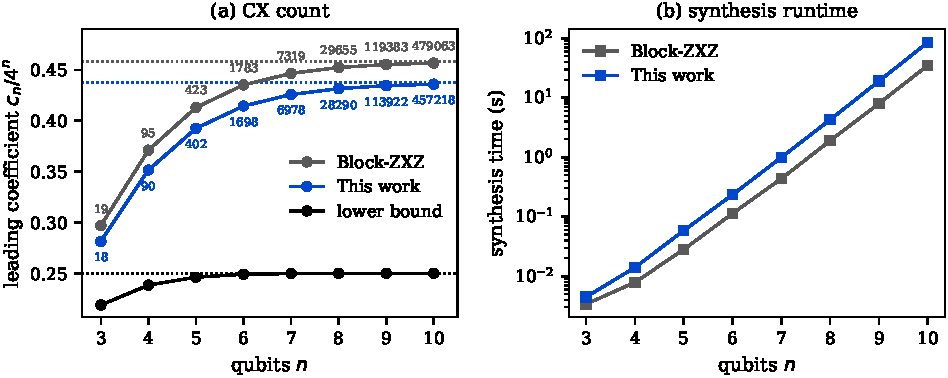
\includegraphics[width=\linewidth]{benchmark.pdf}
\caption{Comparison of the pivot decomposition (blue) with Block-ZXZ (gray).
(a) The CX count divided by $4^n$ (solid dots) with the asymptotic coefficients (dotted lines). Each point is labeled with its CX count.
(b) Total runtime of the decomposition.}
\label{fig:benchmark}
\end{figure}

The pivot decomposition produces quantum circuits using $(4^{n-2}-1)/3$ fewer CX gates at the cost of added runtime. The counts reported in Fig.~\ref{fig:benchmark}a match the expected recurrence formula.

Each recursive step already costs $O(d^3)$, and each root-search iteration also costs $O(d^3)$, so the overhead should be constant as long as the number of iterations does not grow with $n$. This depends on convergence tolerance and warrants further study: the empirical overhead in Fig.~\ref{fig:benchmark}b is about $2$--$2.5\times$. The CX count is independent of the root-search method, so further runtime improvements may be possible.

A second pivot applied in reverse to the right-side multiplexor could perhaps save another
$(4^{n-2}-1)/3$ CX gates, although the two pivots are coupled and would require a joint search.

\section*{Acknowledgements}

Under my supervision, Claude Opus 5.5 (Anthropic) was used to construct all \texttt{Lean} formalisms, generate the numerical experiments, and aid in writing this paper.

\section*{Code availability}

The formal theorems and proofs of the results outlined in Sec.~\ref{sec:alg} and numerical experiments presented in Sec.~\ref{sec:res}
are available~\cite{code}.

\begin{thebibliography}{9}
\bibitem{smb2q} V.~V.~Shende, I.~L.~Markov, S.~S.~Bullock, \emph{Minimal universal two-qubit
controlled-NOT-based circuits}, Phys.\ Rev.\ A 69, 062321 (2004), arXiv:quant-ph/0308033.
\bibitem{smb} V.~V.~Shende, S.~S.~Bullock, I.~L.~Markov, \emph{Synthesis of quantum logic
circuits}, IEEE TCAD 25, 1000 (2006), arXiv:quant-ph/0406176.
\bibitem{zxz} A.~M.~Krol, Z.~Al-Ars, \emph{Beyond quantum Shannon decomposition: circuit
construction for $n$-qubit gates based on block-ZXZ decomposition}, Phys.\ Rev.\ Applied 22,
034019 (2024), arXiv:2403.13692.
\bibitem{baqc} L.~Madden, A.~Simonetto, \emph{Best approximate quantum compiling problems},
ACM Trans.\ Quantum Comput.\ 3, 7 (2022), arXiv:2106.05649.
\bibitem{squander} P.~Rakyta, Z.~Zimbor\'as, \emph{Approaching the theoretical limit in quantum
gate decomposition}, Quantum 6, 710 (2022), arXiv:2109.06770.
\bibitem{mottonen} M.~M\"ott\"onen, J.~J.~Vartiainen, V.~Bergholm, M.~M.~Salomaa,
\emph{Quantum circuits for general multiqubit gates}, Phys.\ Rev.\ Lett.\ 93, 130502 (2004),
arXiv:quant-ph/0404089.
\bibitem{code} M.~Bowring, \emph{lean-unitary}, \url{https://github.com/bowrango/lean-unitary}.
\bibitem{smbdiag} V.~V.~Shende, S.~S.~Bullock, I.~L.~Markov, \emph{Recognizing small-circuit
structure in two-qubit operators and timing Hamiltonians to compute controlled-not gates}, Phys.\ Rev.\ A 70, 012310 (2004), arXiv:quant-ph/0308045.
\end{thebibliography}

\end{document}
